\chapter{Supervised Approach}
qua vengono presentati sia il metodo multilabel classifier GMM-UBM SVM (ESWN) che 
il binary  GMM-UBM SVM (WIRN2016)



\section{Support-Vector Machine based algorithm for evens fall classification}
\label{sec:algorithm_svm_multiclass}
The fall detection task consists in recognize which object produced the pattern of a signal and it mainly consists of two subtasks: the location of the time boundaries of the fall event and the classification of that event. In this section, we concentrate on the second subtask, since the main objective is determining the performance of the acoustic sensor as compared to common aerial microphones. The entire falls detection activity will be addressed in the works presented below.

The fall classification algorithm is composed of a feature extraction stage and a classification stage. The first extracts MFCCs from the input audio signal, while the second classifies the audio event by means of Gaussian means supervectors and SVM. Following is a detailed description of the two stages.

\subsection{Feature extraction}\label{ssec:fx}
Despite MFCCs were originally developed for speech and speaker recognition tasks, they have been successfully applied also for acoustic event classification \cite{Temko2009} and fall detection \cite{zigel2009method}.

\begin{figure}[b]
	\centering
	\includegraphics[width=0.75\columnwidth]{img/mfcc_bn.pdf}
	\caption{The MFCC feature extraction pipeline.} \label{fig:mfcc}
\end{figure}

The block-scheme of the MFCC feature extraction pipeline is shown in \figref{fig:mfcc}. The first processing step is the pre-emphasis of the input signal, which consists in applying a filter whose transfer function is:
\begin{equation}
G(z) = 1 - \alpha z^{-1}.
\end{equation}
Usually $0.9<\alpha\leq1.0$ and here it has been set to 0.97. The objective of pre-emphasis is to remove the DC components and to raise the high-frequency part of the spectrum.

The signal is then segmented in frames 16\,ms long overlapped by 8\,ms and multiplied with a Hamming window. For each frame, the Discrete Fourier Transform (DFT) is calculated and filtered with a filterbank composed of 29 triangular filters uniformly spaced on the mel scale. 

Denoting with $S(i)$ the DFT of a frame and $i$ the frequency bin, the output of the ``Mel Filterbank \& Frequency Integration'' block in \figref{fig:mfcc} is
\begin{equation}
mel(k) = \sum_{i=ini(k)}^{end(k)}|S(i)|^2 W_k(i), \qquad k=1,2,\ldots,N
\end{equation}
where $mel(k)$ is the energy of the $k$-th subband, $W_k(i)$ is the frequency response of the $k$-th filter, $ini(k)$ and $end(k)$ are starting and ending frequency indices of that filter and $N$ is the number of filters in the bank, which in this case is 29. The terms $mel(k)$ are often named ``mel coefficients''.

The final steps for the calculation of the $j$-th MFCC $c(j)$ is the logarithm and the Discrete Cosine Transform (DCT):
\begin{equation}
\begin{aligned}
c(j) = \sum_{k=1}^{N}\log \left[ H(k)\right] \cos\left[\frac{\pi j}{N}(k-0.5)\right], \quad j=0,1,\ldots,M-1\leq N
\end{aligned}
\end{equation}
The set $\{c(0),c(1),\ldots,c(M-1)\}$ forms the static coefficients elements of the feature vector. Here $M$ has been set to 13. The final feature vector is composed of 39 coefficients, i.e., the 13 static coefficients plus their first and second derivatives. %  MFCCs have been extracted with the HCopy tool of the Hidden Markov Model Toolkit \cite{Young2006}.

%Cepstral Mean Normalization (CMN) is then applied to MFCCs to increase the robustness against channel distortions. CMN consists in subtracting the mean of each cepstral coefficients calculated over the entire event:
%\begin{equation}
%c'_t(n) = c_t(n) - \frac{1}{T}\sum_{l=0}^{T-1}c_l(n), \qquad t=0,1,\ldots,T-1
%\end{equation}
%where $t$ denotes the time frame index and $T$ is the event length in frames.

\subsection{Classification stage}
\label{sec:svm_multi_classification}
The approach proposed in this section is based on a One-Class Support Vector Machine (OCSVM) \cite{scholkopf2000}. The general idea is that a human fall produces a sound considerably different from the ones commonly occurring in a home (e.g., voices, sounds from electronic devices, footsteps, etc.). The OCSVM is trained on a large set of ``normal'' sounds to detect acoustic events that deviate from normality. However, it is expected that certain acoustic events are as abnormal as a human fall (e.g., the fall of book, a chair, etc.), thus they could raise false alarms. 



The classification stage employs Gaussian Mean Supervectors (GMS) and a Support Vector Machine classifier as in speaker recognition systems \cite{kinnunen10}. The algorithms consists in modelling the entire acoustic space with a Universal Background Model (UBM) represented by mixture of gaussians (Gaussian Mixture Model, GMM). The GMM is trained using the Expectation Maximization (EM) algorithm \cite{bilmes1998gentle} on a large corpus of acoustic events. Then, for each acoustic event class in the training corpus a GMS is calculated by adapting the UBM with the Maximum A Posteriori (MAP) algorithm \cite{reynolds10} and concatenating the adapted GMM mean values. The block diagram of the approach is shown in \figref{fig:gms}. The final step of the training phase is the estimation of the SVM parameters. In this work, an SVM with a radial basis function has been used. The complete diagram of the training phase is shown in \figref{fig:training-scheme}.

Classification is performed by extracting the supervector from an input audio signal as in the training phase, and then determining the acoustic event class evaluating the SVM discriminant function (\figref{fig:scheme-classify-color}). Since the number of classes is greater than two and SVMs are binary classifiers, the ``one versus all''  technique has been adopted \cite{bishop06}. LIBSVM \cite{chang11} has been employed both in the training and testing phases of the SVM.

\begin{figure}[t]
	\centering
	\includegraphics[width=0.75\columnwidth]{img/gms_bn.pdf}
	\caption{Block scheme for extracting a gaussian mean supervector from MFCCs and a trained UBM.} \label{fig:gms}
\end{figure}

\begin{figure}[t]
	\centering
	\includegraphics[width=0.3334\columnwidth]{img/training_scheme.pdf}
	\caption{Block scheme for training the UBM and SVM models.}
	\label{fig:training-scheme}
\end{figure}

\begin{figure}[t]
	\centering
	
\includegraphics[width=0.333\columnwidth]{img/scheme_classify_bn.pdf}
	\caption{Block-scheme of the fall classification phase.}
	\label{fig:scheme-classify-color}
\end{figure}

\section{Experiments}\label{sec:experiments}

This section firstly presents presents which portion of the dataset described in \secref{sec:dataset} has been used in this work, then the classification performance of the algorithm. 

\subsection{Dataset}
\label{sec:dataset_svm_multiclass}
All the experiments have been conducted data related to R0 room only. In particular, in order to compare the performance of the FAS with a standard aerial microphone, not all data concerning all the aerial microphones array have been used but only the one of the microphone closest to the wall (see \figref{fig:room}). Moreover, signals have been downsampled to 16\,kHz and the resolution has been reduced to 16\,bit. In order to obtain a balanced dataset, for each object and
for each distance, 11 fall events have been randomly picked for a total of 44 events per
object, while all the 44 simulated human fall with the manikin has been selected. In addition, the three musical track recored in the R0 room have been employed to create a noisy version of
the dataset by digitally adding a random segment of the recorded musical tracks
to the ``clean'' datasets as was done for the analysis of the signals in \secref{ssec:sig_analysis}. In particular, the analysis presented in \secref{ssec:sig_analysis} suggested the authors that the standard MFCC extraction pipeline can be modified in order to better exploit the properties the floor acoustic sensor. In particular, the analysis led to the following considerations:
\begin{itemize}
	\item The pre-emphasis filter is an inheritance of automatic speech recognition systems, where the input signal is the human voice. Since the effect of the filter is to enhance the high frequency components of the signal and the floor sensor is more sensitive to low frequencies, removing the pre-emphasis could improve the classification performance.
	\item The majority of the energy of the signals acquired with the floor acoustic sensor is concentrated at frequencies below 1.5\,kHz. This suggest that introducing a low-pass filter that removes low SNR frequencies may improve the classification performance.
\end{itemize}
In \tableref{tab:eswa_dataset} the data used for this approach are summarized.
\begin{table}[t]
	\caption{Data related to R0 room used in this work.}
	\label{tab:eswa_dataset}
	\begin{center}
		\begin{tabular}[t]{c|c}
			
			\hline
			\textbf{Classes}  & \textbf{Nr. of occurrences} \\ %\cline{2-5} 
			%& \hspace{8pt}Clean\hspace{8pt}  & \hspace{6pt}Clean\hspace{6pt}   \\ 
			\hline
			
			Basket      			&   44    	\\
			Fork        			&   44     	\\
			Ball       				&   44    	\\
			Book        			&   44    	\\
			Bag         			&   44    	\\
			Chair       			&   44    	\\
			$\,$ Manikin Doll $\,$ 	&   44    	\\
			\hline
			\textbf{Backgrounds} & \textbf{Total length (s)}\\			
			%			Human Activity  		& 1135  &   3050&   580   	\\
			%			Music					& 1395  &	4330&   3345  	\\
			%			Television				& 0   	&	1675&   1625  	\\
			Classic Music  			&   882   	\\
			Rock Music  			&   616   	\\
			\hline
		\end{tabular}
	\end{center}
\end{table}

\subsection{Experimental setup}
The MFCC extraction pipeline has been firstly parametrised as described in \secref{ssec:fx}, then, based on the study presented in the previous section, two additional pipelines have been tested:
\begin{itemize}
	\item no pre-emphasis (NOPRE): the pre-emphasis stage has been removed from the feature extraction pipeline;
	\item no pre-emphasis plus low-pass filtering (NOPRELP): the pre-emphasis stage has been removed and the maximum frequency of the mel filterbank has been set to 4\,kHz.
\end{itemize}
The standard MFCC extraction pipeline described in \secref{ssec:fx} will be denoted with ``STD'' in the results.

Regarding the UBM, it has been trained until convergence with the EM algorithm setting the threshold value to $10^{-3}$. The same value has been employed in the MAP adaptation algorithm, but the maximum number of iterations was set to 5.

Due to the limited amount of data, the experiments have been conducted with the leave-one-label-out method: fall events recorded at all distances but one were employed for training and validation, while the remaining for testing. The validation phase consisted in searching for the number of components of the UBM and for the SVM hyperparameters which yielded the best results. In particular, the number of components of the UBM assumed the values $\{ 1,2,\ldots,64 \}$, while the SVM hyperparameters $C$ and $\gamma$ the values $\{ 2^{-5},2^{-3},\ldots,2^{15} \}$ and $\{ 2^{-15},2^{-13},\ldots,2^{3} \}$ respectively. 

The performance was evaluated both on clean data and on data corrupted with the music interference. In particular, the system was evaluated in matched condition, where the acoustic scenario of the training, validation and test data is the same, in mismatched condition, where training data is clean and testing data is corrupted with music, and in multi-condition, where training data and testing data contain both clean signals and corrupted signals. In the latter case, the training, validation and test sets have been divided so that they contain 1/3 of clean data and 2/3 of noisy data.

The performance has been evaluated in terms of precision ($P$), recall ($R$) and F$_1$-Measure ($F$) per class and the values have then been averaged. The metrics definitions for class $i$ is:
\begin{align}
P_i &=  \frac{C(i,i) }{\sum_j C(j,i)}, \\
R_i &=  \frac{C(i,i) }{\sum_j C(i,j)}, \\
F_{i} &= \frac{2P_iR_i}{P_i+R_i},
\end{align}
where $C=[C(i,j)]$ is the confusion matrix.

%\begin{table}[t]
%\centering
%\caption{Number of fall events employed for training, validation and testing. \textbf{@Diego: completare.}}\label{tbl:tvtsplit}
%\begin{footnotesize}
%\begin{tabular}{r | c c c c c c c | c}
%\hline						 
%						 & \textbf{Volleyball} & \textbf{Basket} & \textbf{Book} & \textbf{Fork} & \textbf{Chair} & \textbf{Bag} & \textbf{Doll} & \textbf{Total} \\						 
%\hline
%\textbf{Training}     & 32 & 32 & 32 & 32 & 48 & 32 & -- &    --      \\
%\textbf{Validation}   & 16 & 16 & 16 & 16 & 24 & 16 & --  &    --         \\
%\textbf{Testing}      & 16 & 16 & 16 & 16 & 24 & 16 & -- &     --        \\
%\hline
%\end{tabular}
%\end{footnotesize}
%\end{table}

%The best performance was obtained by using an UBM with 16 mixtures, $C=\{2,2,2^{-1},2\}$ and $\gamma=\{2^{-9},2^{-9},2^{-7},2^{-7} \}$. The values of $C$ and $\gamma$ are four since they are specific for each test fold.

\subsection{Results in matched condition}
\figref{fig:results_match} shows the results obtained in matched condition. As shown in the figure, the FAS exceeds the F$_1$-Measure of the aerial microphone both with clean and noisy signals regardless the feature setup employed. In particular, in clean conditions the aerial microphone achieves the highest F$_1$-Measure with standard MFCCs, while the FAS with the NOPRELP ones, which results in 6.50\% absolute improvement. In noisy conditions, the aerial microphones best performance is again achieved with STD features, while the FAS one is achieved with the NOPRE features, with the NOPRELP setup performing almost the same. The absolute improvement of the FAS respect to the aerial microphone is 5.36\%.

\begin{figure}[t]
	\centering
	\begin{subfigure}[b]{0.6\textwidth}
		\includegraphics[width=\textwidth]{img/pgfsources/16_matched_clean/16_matched_CLEAN.pdf}
		\caption{}\label{fig:results_match_clean}
	\end{subfigure}
	\begin{subfigure}[b]{0.6\textwidth}
		\includegraphics[width=\textwidth]{img/pgfsources/16_matched_noisy/16_matched_NOISY.pdf}
		\caption{}\label{fig:results_match_noisy}
	\end{subfigure}
	\caption{Fall classification performance in matched condition with clean (a) and noisy signals (b).} \label{fig:results_match}
\end{figure}

Focusing on the FAS performance with the various feature extraction pipelines, the highest F$_1$-Measure is obtained by removing the pre-emphasis and low-pass filtering the signals (NOPRELP) in clean conditions. Notice, however, the standard pipeline performs almost the same, thus in this condition the influence is minimal. The sole removal of the pre-emphasis, on the other hand, is detrimental for the classification performance. The opposite occurs in noisy condition, where the removal of the pre-emphasis improves the results by 3.99\%. Low-pass filtering, on the other hand, does not give further improvements. Overall, the feature pipeline that gives the highest F$_1$-Measure is the NOPRELP, as argued in \secref{ssec:sig_analysis}.

Further insights on the results are given by the confusion matrices of the aerial microphone (\tableref{tbl:cm_mic_clean_matched_np}) and of the FAS (\tableref{tbl:cm_fas_clean_matched_npre4k}) for the feature pipeline giving the highest F$_1$-Measure. With the only exception of the basket falls, the FAS is able to achieve superior performance for all the objects in the dataset. In particular, the doll F$_1$-Measure improves by 9.89\% respect to the aerial microphone. The object exhibiting the lowest performance regardless the sensor is the book: this can denote a limit in the algorithm suggesting that further improvements could be obtained by properly modifying the features or the classifier.

\begin{table}[t]
	\caption{Aerial microphone confusion matrix related to the STD configuration in clean condition. The average precision is 91.48\%, the average recall 91.23\%, and the average F$_1$-Measure 91.04\%.}
	\label{tbl:cm_mic_clean_matched_np}
	\centering
	\footnotesize
	\begin{tabular} {r  *{7}{E} | c|}
		\hhline{~*{8}-}
		\multicolumn{1}{c}{} & \multicolumn{1}{|c}{\textbf{Doll}} & \multicolumn{1}{c}{\textbf{Bag}} & \multicolumn{1}{c}{\textbf{Ball}} & \multicolumn{1}{c}{\textbf{Basket}} & \multicolumn{1}{c}{\textbf{Book}} & \multicolumn{1}{c}{\textbf{Chair}} & \multicolumn{1}{c|}{\textbf{Fork}} 
		& \multicolumn{1}{c|}{\textbf{F$_1$}}\\
		\hhline{*{9}{-|}}
		\multicolumn{1}{|r|}{~\textbf{Doll}} & 93.18 & 0 & 0 & 0 & 2.27 & 4.55 & 0 & 90.11 \\ 
		\multicolumn{1}{|r|}{~\textbf{Bag}} & 0 & 86.36 & 0 & 0 & 13.64 & 0 & 0 & 82.61 \\
		\multicolumn{1}{|r|}{~\textbf{Ball}} & 0 & 0 & 100.00 & 0 & 0 & 0 & 0 & 100.00 \\  
		\multicolumn{1}{|r|}{~\textbf{Basket}} & 2.27 & 0 & 0 & 97.73 & 0 & 0 & 0 & 98.85 \\ %\hline
		\multicolumn{1}{|r|}{~\textbf{Book}} & 0 & 22.73 & 0 & 0 & 77.27 & 0 & 0 & 78.16\\ %hline
		\multicolumn{1}{|r|}{~\textbf{Chair}} & 11.36 & 0 & 0 & 0 & 4.55 & 84.09 & 0 & 89.16 \\ %\hline
		\multicolumn{1}{|r|}{~\textbf{Fork}} & 0 & 0 & 0 & 0 & 0 & 0 & 100 & 100.00\\ \hhline{*{9}{-}}
		\multicolumn{1}{|r|}{~\textbf{Precision}} & \multicolumn{1}{c}{87.27} & \multicolumn{1}{c}{79.17} & \multicolumn{1}{c}{100.00} & \multicolumn{1}{c}{100.00} & \multicolumn{1}{c}{79.07} & \multicolumn{1}{c}{94.87} & \multicolumn{1}{c|}{100.00} & \multicolumn{1}{c}{} \\ \hhline{*{8}{-}}
	\end{tabular}
\end{table}

\begin{table}[t]
	\caption{FAS confusion matrix related to the NPRELP configuration in clean condition. The average precision is 98.13\%, the average recall 98.05\%, and the average F$_1$-Measure 98.06\%.} 
	\label{tbl:cm_fas_clean_matched_npre4k}
	\centering
	\footnotesize
	\begin{tabular} {r  *{7}{E} | c|}
		\hhline{~*{8}-}
		\multicolumn{1}{c}{} & \multicolumn{1}{|c}{\textbf{Doll}} & \multicolumn{1}{c}{\textbf{Bag}} & \multicolumn{1}{c}{\textbf{Ball}} & \multicolumn{1}{c}{\textbf{Basket}} & \multicolumn{1}{c}{\textbf{Book}} & \multicolumn{1}{c}{\textbf{Chair}} & \multicolumn{1}{c|}{\textbf{Fork}} 
		& \multicolumn{1}{c|}{\textbf{F$_1$}}\\
		\hhline{*{9}{-|}}
		\multicolumn{1}{|r|}{~\textbf{Doll}} & 100.00 & 0 & 0 & 0 & 0 & 0 & 0& 100.00 \\ 
		\multicolumn{1}{|r|}{~\textbf{Bag}} & 0 & 97.73 & 0 & 0 & 2.27 & 0 & 0& 97.73 \\ 
		\multicolumn{1}{|r|}{~\textbf{Ball}} & 0 & 0 & 100.00 & 0 & 0 & 0 & 0  & 100.00 \\   
		\multicolumn{1}{|r|}{~\textbf{Basket}} &  0 & 0 & 0 & 95.45 & 2.27 & 2.27 & 0 & 97.67 \\  %\hline
		\multicolumn{1}{|r|}{~\textbf{Book}} &  0 & 2.27 & 0 & 0 & 97.73 & 0 & 0 & 94.51 \\  %hline
		\multicolumn{1}{|r|}{~\textbf{Chair}} & 0 & 0 & 0 & 0 & 4.55 & 95.45 & 0  & 96.55 \\  %\hline
		\multicolumn{1}{|r|}{~\textbf{Fork}} & 0 & 0 & 0 & 0 & 0 & 0 & 100.00  & 100.00 \\   \hhline{*{9}{-}}
		\multicolumn{1}{|r|}{~\textbf{Precision}} & \multicolumn{1}{c}{100.00} & \multicolumn{1}{c}{97.73} & \multicolumn{1}{c}{100.00} & \multicolumn{1}{c}{100.00} & \multicolumn{1}{c}{91.49} & \multicolumn{1}{c}{97.67} & \multicolumn{1}{c|}{100.00} & \multicolumn{1}{c}{} \\ \hhline{*{8}{-}}
	\end{tabular}
\end{table}

\subsection{Results in mismatched condition}
\figref{fig:results_mismatch} shows the results obtained in mismatched condition, i.e., with training and validation performed on clean data and testing on noisy data. As expected, both the performance of the aerial microphone and of the floor sensor decrease. Notice, however, that regardless the features employed, the floor sensor is able to achieve considerably higher F$_1$-Measures respect to the aerial microphone. In particular, the floor sensor highest F$_1$-Measure, obtained with the NPRE features, exceeds the one of the aerial microphone obtained with the standard MFCC pipeline by 8.76\%. This value confirms that the higher SNR of the floor sensor signals actually results in better classification performance.

Regarding the features, the hypothesis that the pre-emphasis could be detrimental for the performance of the sensor is confirmed: indeed, the highest F$_1$-Measure has been obtained with the NOPRE configuration and exceeds the one of the standard MFCC pipeline by 1.32\%. Differently, the introduction of the low-pass filter does not result in better performance respect to the NOPRE case. %The motivation is probably that despite being noisy, the information contained in the higher frequencies is still relevant for classification.

\begin{figure}[t]
	\centering
	\includegraphics[width=0.75\textwidth]{img/pgfsources/16_mismatched/16_mismatched}
	\caption{Fall classification performance in mismatched condition.} \label{fig:results_mismatch}
\end{figure}

\subsection{Results in multicondition}
\figref{fig:results_multi} shows the results obtained in multicondition, i.e., when training and test sets both contain clean and noisy data. The results further confirm the superiority of the FAS respect to the aerial microphone, with the first reaching 90.82\% using the NOPRE features and the latter reaching 85.28\% using the standard MFCC pipeline. Regarding the features, \figref{fig:results_multi} confirms that removing the pre-emphasis indeed improves classification results, while introducing the low-pass filtering does not give further benefits.

\begin{figure}[t]
	\centering
	\includegraphics[width=0.75\textwidth]{img/pgfsources/16_multicondition/16_multicondition}
	\caption{Fall classification performance in multicondition.} \label{fig:results_multi}
\end{figure}

\subsection{Final remarks}
The experimental results taken as a whole provide important insights on the system behavior and allow us to express possible future directions for its improvement. In particular, the experiments demonstrated the superiority of the floor acoustic sensor compared to the aerial microphone. The results in matched condition are notable, since the F$_1$-Measure is greater than 98\% in clean condition and close to 90\% in noisy condition. The experiment in matched condition is important to compare the performance of the two sensors, but it puts the classifier in a favourable scenario. The mismatched condition is closer to a real scenario, where the classifier is trained on a dataset whose characteristics differ from testing ones. The floor sensor still achieves higher results compared to the aerial microphone, but respect to the matched condition they are considerably lower. This suggests that there is room for improvement both on the sensor side and on the algorithmic side.

Regarding the sensor, the insertion of isolating material in the enclosure would further reduce the impact of external interferences. On the algorithmic side, different low-level features could be employed instead of MFCCs. In particular, recalling the works on speech recognition systems, Power Normalized Cepstral Coefficients (PNCCs) \cite{Kim12} exhibited good performance in noisy conditions and could be considered also for fall classification. In addition, the SVM classifier here employed has not been designed to recognize a specific class. In the latter case, e.g., focusing on the human fall class, the problem can be tackled in two ways: as a two class problem, where one class is the class of interest and the other comprises ``the rest of the world'' that will be addressed in \secref{sec:biclass_svm} or as a novelty detection problem, where the ``novel'' events are represented by the specific class occurrence that will be addressed in \secref{sec:ocsvm}. In both cases, the classification task is simpler, since the number of classes to discriminate is reduced and the overall performance is expected to increase \cite{bishop06}.

\section{Binary SVM based classifier for human fall detection}
\label{sec:biclass_svm}

The classification algorithm is based on the previous work. It employs both low-level features, i.e., MFCCs \cite{Davis80}, and high-level features, i.e., Gaussian Mean Supervectors which are then used by a Support Vector Machine to distinguish falls from no-falls. Despite MFCCs were originally developed for speech and speaker recognition tasks, they have been successfully applied also for acoustic event classification \cite{Temko06} and fall detection \cite{zigel2009method}. Differently from the algorithm presented in the previous section, where the algorithm discriminated falls of general objects, here the focus is specifically on the classification of human falls. The classifier, thus, has been designed to discriminate between two classes: human falls and generic sound events. In order to assess the performance of the approach, the dataset described in \secref{sec:dataset_svm_multiclass} has been augmented with instances of everyday sounds (speech, footsteps, etc.), thus making the task more challenging. As a reference, results employing the original dataset (\secref{sec:dataset_svm_multiclass}) are also reported.

The classification algorithm is composed of two main parts.
The first is the features extraction phase where we have extract the Mel Frequency Cepstral Coefficients from all audio files that comprise the dataset. For doing this, the feature extraction pipeline is the same used in \secref{ssec:fx}. In particular, the signal is segmented in frames 16\,ms long overlapped by 8\,ms, the parameter $\alpha$ of the pre-emphasis filter has been set to 0.97 and the number of filters which compose the filterbank has been set to 29. At the end, after the Discrete Cosine Transform, 13 statics coefficients are extracted that, together with their first and second derivatives, form the final feature vector of a signal.

The classification phase is similar to that one adopted in \secref{sec:svm_multi_classification}: first it uses a mixture of gaussians (GMM), trained on a large corpus of audio events with the Expectation Maximization algorithm to model the acoustic space (Universal Background Model, UBM). Then, for each audio segment, the Maximum a Posteriori (MAP) algorithm is used to calculate the Gaussian Mean Supervector (GMS) from the MFCCs. %The GMSs are then employed in validation phase to estimate the Support Vector Machine parameters.
%a MAP algorithm is employed to model the acoustic space with Universal Background Model (UBM),  starting from the MFCCs.  calculate the Gaussian Mean Supervector (GMN) starting from the MFCC using the GMM-UBM paradigm, then estimate the SVM parameters. 
In contrast with the previous work \secref{sec:svm_multi_classification}, where we used a multi-class approach, here we employ a binary SVM to discriminate the class ``fall'' from ``rest'' which allows to distinguish human falls from the other types of sounds. In addition, the class decision is usually performed by evaluating the sign of the SVM discriminative function, which ultimately consists in deciding whether in example belongs to a class by setting a threshold equal to zero. However, in a human fall classification task, it is important to minimize the probability of missing a fall event, i.e., false negatives. In order to push the system towards this direction, we decided to consider the entire value of the SVM discriminative function, and then to set an appropriate threshold in order to minimize the occurrence of false negatives.

\subsection{Dataset}\label{sec:data_binary_svm}

As can be seen in the \tableref{tab:binary_svm_dataset}, the dataset used for training and assess the proposed method is an enlarged version of the one used in \secref{sec:algorithm_svm_multiclass}. Moreover, in order to further stress the system, a 20 minutes long recording session in which 2 persons have produced everyday noises such as talking, walking, dragging chairs, and playing with the ball was used. Then the track obtained in this session has been divided in 665 sub-tracks. The lengths of these sub-tracks have been randomly generated with gaussian distribution. Mean value and standard deviation of this distribution have been calculated based on the lengths of the other files that form the dataset. 
In addition to the clean dataset, a noisy version has been created to assess the performance in noisy condition. The noisy dataset consists in a musical background recorded with both sensors and digitally added to the clean events.


\begin{table}[t]
	\caption{Data related to R0 room used in this work.}
	\label{tab:binary_svm_dataset}
	\begin{center}
		\begin{tabular}[t]{c|c}
			
			\hline
			\textbf{Classes}  & \textbf{Nr. of occurrences} \\ %\cline{2-5} 

			\hline
			
			Basket      			&   44    	\\
			Fork        			&   44     	\\
			Ball       				&   44    	\\
			Book        			&   44    	\\
			Bag         			&   44    	\\
			Chair       			&   44    	\\
			$\,$ Manikin Doll $\,$ 	&   44    	\\
			\hline
			\textbf{Backgrounds} & \textbf{Total length (s)}\\			
			%			Human Activity  		& 1135  &   3050&   580   	\\
			%			Music					& 1395  &	4330&   3345  	\\
			%			Television				& 0   	&	1675&   1625  	\\
			Classic Music  			&   882   	\\
			Rock Music  			&   616   	\\
			human activities 		&   665		\\
			\hline
		\end{tabular}
	\end{center}
\end{table}

\subsection{Experiments}\label{sec:exp}
%\vspace{-0.10cm}
In this section, the experimental procedure is firstly discussed and then the algorithm performance is presented. In the experiments, the signals of the dataset described above have been downsampled to 8\,kHz and the bit depth has been reduced to 16 bit. Both the choice of the sampling frequency and the choice of MFCCs are justified by the analysis performed in the \secref{ssec:sig_analysis}, where it was shown that the signals recorded with the FAS have the majority of the energy concentrated at low frequencies (below 1\,kHz). Indeed, the mel scale used in the feature extraction pipeline has a higher resolution at low frequencies, that allows to better describe the portion of the spectrum where the majority of the energy resides. In addition, the algorithm has been evaluated using two features extraction pipelines:
\begin{itemize}
	\item the first is the same described in the \secref{ssec:fx} and will be denoted as STD; %and it will later be called by the abbreviation STD (standard) 
	\item the second pipeline does not include the pre-emphasis filter and will be denoted with NOPRE.
\end{itemize}

The experiments have been conducted with a 4-fold cross-validation strategy and a three-way data split in three different operating conditions:
\begin{itemize}
	\item matched, where the training, validation and test sets share the same acoustic condition, i.e., clean or noisy;
	\item mismatched, where the training set is composed of clean signals while the validation and test sets are composed of noisy signals;
	\item multicondition, where the training, validation and test sets contain both clean and noisy data. In this case the sets have been divided so that they contain 1/3 of clean data and 2/3 of noisy data.
\end{itemize}

The tests have been conducted also without using the signals of everyday noises, i.e., using the same dataset employed in \secref{sec:dataset_svm_multiclass}. The performance is evaluated in terms of F$_1$-Measure per class and the values have then been averaged to obtain a single performance metric. To better describe the algorithm behavior, we have used the Detection Error Trade-off (DET) curve, as defined in \cite{Martin97}. This graph allows evaluating the false alarm probability when miss probability is equal to 0 (henceforward named as FPM0), which is particularly relevant in a fall classification task.


\subsubsection{Results in matched condition}
%\vspace{-0.25cm}
\figref{fig:match_bck} shows the results obtained in the matched condition case study using the enlarged version of the dataset. In \figref{fig:match_bck_BAR}, the FAS achieves higher F$_1$-Measures both in clean and noisy conditions. In the first case, the floor sensor exceeds the F$_1$-Measure of the aerial microphone obtained with the standard MFCC pipeline by 0.11\%. In the noisy condition case study, the FAS with STD features achieves an F$_1$-Measure greater than 0.3\% with respect to the aerial microphone with NOPRE features.

\begin{figure}[t]
	\centering
	\begin{subfigure}[b]{0.6\textwidth}
		\includegraphics[width=\textwidth]{img/winr2016/pgfsource/8_bck_matched/BAR_8_bck_matched.pdf}
		\caption{F$_1$-Measure histogram plot.}\label{fig:match_bck_BAR}
	\end{subfigure}
	\hspace{5mm}
	\begin{subfigure}[b]{0.6\textwidth}
		\includegraphics[width=\textwidth]{img/winr2016/matlab2tikz/8_bck_matched/DET_8_bck_matched.pdf}
		\caption{ Comparison of DET graphs.}\label{fig:match_bck_DET}
	\end{subfigure}
	\caption{Fall classification performance in matched condition with the dataset comprising everyday noises.}\label{fig:match_bck}

\end{figure}

The DET curves are shown in \figref{fig:match_bck_DET}. Note that the lines relative to the FAS in clean condition are both absent. This is because independently from the threshold, either the miss probability or the false alarm probability is 0 and the DET curves assume  values towards minus infinite (in logarithmic scale). This means that the FPM0 are 0 for both these configurations, while the lower FPM0 for the aerial microphone in clean condition is 1.3\%. Regarding the tests with noisy signals, the performance difference between the two sensors increases, since the FPM0 is equal to 2.2\% with the FAS (NOPRE) and is equal to 12.5\% with the aerial sensor (STD).

In order to facilitate the analysis, \tableref{tab:match_lolo44} summarises the results obtained with the dataset version used in \secref{sec:dataset_svm_multiclass}, which does not comprise everyday noises. As it can be observed, with respect to the previous results, the performance decreases in all tests and for both the F$_1$-Measure and the FPM0, although the gap between the FAS and the aerial microphone increases.

\subsubsection{Results in mismatched condition}

The mismatched condition  is the most difficult case for the classifier. As expected, the performance decrease for both sensors. Focusing on \figref{fig:mism_bck_BAR}, the best F$_1$-Measure is obtained with the NOPRE pipeline for both the FAS and aerial microphone, and is equal to 99.14\% and 98.43\% respectively. A consistent performance difference between the two sensors can be observed in \figref{fig:mism_bck_DET}, where the smallest FPM0 for the FAS, obtained with NOPRE, is around 13\% while for the aerial one is 95\%, this time obtained with STD.

\begin{figure}[t]
	\centering
	\begin{subfigure}[b]{0.6\textwidth}
		\includegraphics[width=\textwidth]{img/winr2016/pgfsource/8_bck_mismatched/BAR_8_bck_mismatched.pdf}
		\caption{F$_1$-Measure histogram plot.}\label{fig:mism_bck_BAR}	
	\end{subfigure}
	\hspace{5mm}
	\begin{subfigure}[b]{0.6\textwidth}
		\includegraphics[width=\textwidth]{img/winr2016/matlab2tikz/8_bck_mismatched/DET_8_bck_mismatched.pdf}
		\caption{Comparison of DET curves.}\label{fig:mism_bck_DET}	
	\end{subfigure}
	\caption{Fall classification performance in mismatched condition with the dataset comprising everyday noises.}

\end{figure}

The results of the mismatched experiments obtained with the dataset without everyday noises are reported in \tableref{tab:mism_lolo44}. Regarding the F$_1$-Measure, a performance decrease can be observed compared to the results in \figref{fig:mism_bck_BAR}. Differently, the aerial microphone FPM0 improves, but it is again below the FPM0 achieved by the FAS with NOPRE MFCCs (12.5\%).


\subsubsection{Results in multicondition}
\figref{fig:multi_bck} shows the results in the multicondition case. The FAS superiority is confirmed, since it achieves an F$_1$-Measure equal to 99.78\% regardless the feature extraction pipeline, while the aerial sensor obtains an F$_1$-Measure equal to 99.19\% with the STD pipeline.

Regarding the DET plot (\figref{fig:multi_bck_DET}), an FPM0 equal to 2.9\% is achieved by the FAS, but differently from the previous cases, with the STD feature. The aerial microphone achieves an FPM0 equal to 9.8\% with the NOPRE pipeline.

\begin{figure}[t]
	\centering
	\begin{subfigure}[b]{0.6\textwidth}
		\includegraphics[width=\textwidth]{img/winr2016/pgfsource/8_bck_multicondition/BAR_8_bck_multicondition.pdf}
		\caption{F$_1$-Measure histogram plot.}\label{fig:multi_bck_BAR}	
	\end{subfigure}
	~
	\begin{subfigure}[b]{0.6\textwidth}
		\includegraphics[width=\textwidth]{img/winr2016/matlab2tikz/8_bck_multicondition/DET_8_bck_multicondition.pdf}
		\caption{Comparison of DET curves.}\label{fig:multi_bck_DET}	
	\end{subfigure}
	\caption{Fall classification performance in multicondition with the dataset comprising everyday noises.}\label{fig:multi_bck}
	\vspace{-0.25cm}
\end{figure}

In the last table (\tableref{tab:multi_lolo44}) are shown the result of the multicondition tests obtained by using the smaller dataset. Again there is an overall decrease for the F$_1$-Measure, greater for the aerial microphone, while the FAS exhibiting a FPM0 equal to 0\% contrary to the increasing FPM0 for the aerial sensor.
\begin{table}[t]
	%\begin{wraptable}[9]{r}[0pt]{6cm} 
	\centering
	\caption{Fall classification performance in matched condition with the dataset excluding everyday noises.}\label{tab:match_lolo44}
	\begin{tabularx}{\textwidth}{ | X  X | X X | X  X | }
		\hline
		&			&\multicolumn{2}{c|}{STD} 	&\multicolumn{2}{c|}{NOPRE}  \\
		&		  	& F$_1$-Measure 		& FPM0 			& F$_1$-Measure & FPM0   \\ \hline
		\multirow{ 2}{*}{Clean} & Aerial  	& 96.29 		 		& 9.85			& 93.11 		 & 4.95	  		\\
		& FAS 	 	& 98.81 		 		& 0.00	  		& 100.00   	 	 & 0.00	   \\ \hline
		\multirow{ 2}{*}{Noisy} & Aerial 	& 97.22 		 		& 43.00   		& 96.92 		 & 73.00  	  \\
		& FAS	 	& 99.63			 		& 6.05   		& 99.62 		 & 9.85  	  \\ \hline
	\end{tabularx}

\end{table} 

\begin{table}[t]
	\centering
	\caption{Fall classification performance in mismatched condition (a) and multicondition (b) with the dataset excluding everyday noises. F$_1$ denotes the F$_1$-Measure.}

	\begin{subtable}[b]{1\textwidth}
		\centering
		\caption{}\label{tab:mism_lolo44}		
		\begin{tabularx}{\textwidth}{ | c  X | X  X | X  X | }
			\hline
			&	\%		&\multicolumn{2}{c|}{STD}					&\multicolumn{2}{c|}{NOPRE}  \\
			&		  	& \hspace{0.15cm}F$_1$	& FPM0 				&\hspace{0.15cm}F$_1$ 	& FPM0   \\ \hline
			& Aerial  	& 96.20 				& 87.50				& 95.44	& 76.00	  		\\
			& FAS 	 	& 97.80 				& 34.50	  			& 98.11 & 12.50	   \\ \hline
			
		\end{tabularx}
	\end{subtable}
	\begin{subtable}[b]{1\textwidth}
		\centering
		\caption{}\label{tab:multi_lolo44}		
		\begin{tabularx}{\textwidth}{ | c X | X  X | X  X | }
			\hline
			&	\%		&\multicolumn{2}{c|}{STD} 					&\multicolumn{2}{c|}{NOPRE}  \\
			&		  	& \hspace{0.15cm}F$_1$	& FPM0 				& \hspace{0.15cm}F$_1$		& FPM0   \\ \hline
			& Aerial  	& 96.80 				& 16.50				& 96.78 	& 31.4	  		\\
			& FAS 	 	& 99.62 				& 0.00				& 99.43  	& 0.00	   \\ \hline
			
		\end{tabularx}
	\end{subtable}

\end{table}
\subsection{Final remarks}
In this section, a human fall classification system based on the previous work discussed in \secref{sec:algorithm_svm_multiclass} has been described. The main sensor used in the FAS the sensor operates similarly to stethoscopes, with a microphone embedded in a resonant enclosure and a membrane in contact with the floor that captures the acoustic waves resulting from a fall. The performance of that sensor has been compared with the one obtained by a standard aerial microphone. The classification algorithm extracts MFCC features from the signal acquired with the FAS, and then discriminates a fall from a generic event by using GMM supervectors and an SVM classifier. Differently from the works discussed in  \secref{sec:algorithm_svm_multiclass}, here we specifically addressed the human fall classification task by designing the classifier to discriminate human falls from other events.

The performance of the system has been evaluated on a corpus containing recordings of several events: falls of a human mimicking doll, falls of common objects and everyday noises (speech, footsteps, etc.). In order to assess the performance of the solution in adverse acoustic conditions, a noisy version of the dataset has been created. The experiments have been performed in three operating conditions: matched, mismatched and multicondition, and the performance has been evaluated in terms of average F$_1$-Measure and false alarm probability when the miss probability is equal to 0. The superiority of the FAS resulted evident in all the addressed conditions, in particular with an F$_1$-Measure equal to 100\%  and an FP0 equal to 0\% in clean matched conditions, and an F$_1$-Measure equal to 99.14\% and an FP0 equal to 13\% in noisy mismatched conditions.

%In addition to the very good F$_1$-Measure performance in all three operative contexts, i.e. matched mismatched and multicondition, and with both the dataset versions, the low probability of the false alarm when the miss probability is equal to 0 reached by the FAS suggests that the proposed solution could be transformed into a commercial product in the near future.
Moreover, by looking at the results obtained with the two different features pipeline, the FAS based solution always show robust performance and it is difficult to determine which represents the best choice. 
The increasing performance (F$_1$-Measure) obtained with the largest version of dataset, in truth, are due to the fact that signals corresponding to the everyday noises are extremely easy to classify 
being very different from a fall.

As future works, the datasets will be expanded in order to evaluate the system performance in case the falls occurs in a different room respect to the FAS one or in different scenario as falls occurs in presence of furniture or with a different paving. Both this aspect will be addressed in \secref{sec:autoencoder_one_shot}. In addition, the detection of the time boundaries of the fall event will be addressed and techniques originally developed for enhancing speech will be evaluated to increase the robustness to acoustic distortions \cite{Rotili08,Cifani2008}.